\section{Mechanism Findings}\label{sec:mechanism}

The headline result of Section~\ref{sec:results} — that in-context
surface forms beat the production KG agents — leaves open
\emph{which} surface form properties drive the gap. Three mechanism
findings, summarized below, refine the picture.

\subsection{Query-Language Familiarity Dominates LLM-Family Effects}

Three of four LLM families are essentially form-agnostic across the
four in-context tiers. The form-by-form spread is 6 percentage
points for HCX-32B-Think (85--91), 3 for Qwen3-235B (90--93), and
4 for gpt-oss-120b (91--95). Llama-4-Scout is the outlier: a
21-percentage-point spread driven by a steep drop on the structured
tiers (C-TQL 63\%, C-Cypher 62\%, C-JSONLD 67\%) while C-NL holds at
83\%. Figure~\ref{fig:form-sensitivity} visualizes the asymmetry.

% Figure: Llama-4 form sensitivity vs other LLMs.
\begin{figure}[t]
\centering
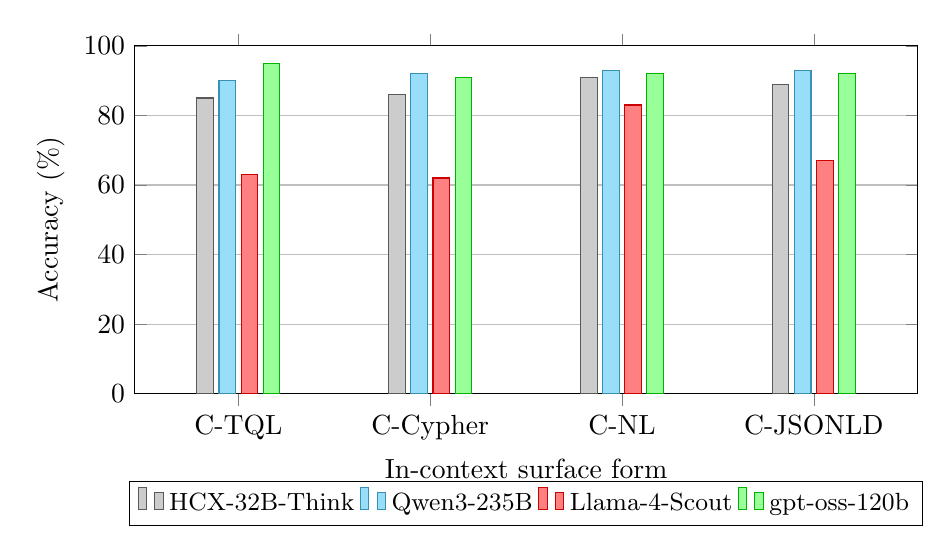
\begin{tikzpicture}
\begin{axis}[
  width=0.95\textwidth,
  height=6cm,
  ybar=2pt,
  bar width=6pt,
  ymin=0, ymax=100,
  ymajorgrids=true,
  ylabel={Accuracy (\%)},
  xlabel={In-context surface form},
  symbolic x coords={C-TQL, C-Cypher, C-NL, C-JSONLD},
  xtick=data,
  legend style={at={(0.5,-0.25)}, anchor=north, legend columns=4, font=\small},
  enlarge x limits=0.18,
]
\addplot[fill=gray!40, draw=gray!70!black] coordinates {
  (C-TQL, 85) (C-Cypher, 86) (C-NL, 91) (C-JSONLD, 89)
};
\addplot[fill=cyan!40, draw=cyan!70!black] coordinates {
  (C-TQL, 90) (C-Cypher, 92) (C-NL, 93) (C-JSONLD, 93)
};
\addplot[fill=red!50, draw=red!80!black] coordinates {
  (C-TQL, 63) (C-Cypher, 62) (C-NL, 83) (C-JSONLD, 67)
};
\addplot[fill=green!40, draw=green!70!black] coordinates {
  (C-TQL, 95) (C-Cypher, 91) (C-NL, 92) (C-JSONLD, 92)
};
\legend{HCX-32B-Think, Qwen3-235B, Llama-4-Scout, gpt-oss-120b}
\end{axis}
\end{tikzpicture}
\caption{In-context surface-form accuracy by LLM family. Three of four
LLMs are essentially form-agnostic (within 8 percentage points across
TQL, Cypher, NL, JSON-LD). Llama-4-Scout exhibits a 21-percentage-point
gap (C-NL 83\% vs.\ C-TQL/Cypher 62--63\%), tracing the bottleneck to
\emph{query-language familiarity in pretraining} rather than the
expressivity of the underlying KG.}
\label{fig:form-sensitivity}
\end{figure}


The asymmetry traces directly to query-language familiarity in the
LLM's pre-training corpus. C-TQL's role-player syntax \texttt{(role1:
\$a, role2: \$b) isa Relation;} appears far less frequently in
public text than Cypher \texttt{CREATE (a)-[:R]->(b)} or JSON-LD,
which is itself less common than English prose. Llama-4-Scout's
weakness on the structured tiers reproduces in production
\backendname{typedb} (56\%), where the agent must in addition
\emph{generate} TQL queries — confirming that the bottleneck is not
the data model but the query-language interface.

\paragraph{Per-category breakdown (Llama-4 C-TQL).}
Within Llama-4's 63\% on C-TQL, the failure modes are not uniform:
single-fact extraction tasks remain strong (\texttt{calculation}
86\%, \texttt{article\_text} 100\%), while cross-reference tasks
collapse (\texttt{comparison} 38\%, \texttt{multihop\_3key} 47\%,
\texttt{aggregation} 50\%, \texttt{negation\_exception} 25\%).
Lookup of one fact survives an unfamiliar syntax; \emph{traversing}
multiple facts under that syntax does not.

\subsection{In-Context KG Underperforms NL on Boundary Inference}

The previous section's mechanism is about \emph{positive}
queries — where the answer exists in the data. A symmetric question
is whether the surface form matters for \emph{negative} queries,
where the correct answer is "no such fact exists." We isolate the
six \texttt{out\_of\_scope} questions: each asks for a
(position, grade), (country, grade), or (allowance) combination
that is provably absent from the regulation tables. For all six
questions the in-context dumps contain enough information to derive
the absence (the position-pay table lists all valid combinations,
the overseas-pay table lists all six countries, and the article-text
prefix defines the closed set of allowances).

% Figure: Out-of-scope category — closed-world boundary inference.
% In-context KG (TQL/Cypher) underperforms NL despite full data coverage.
\begin{figure}[t]
\centering
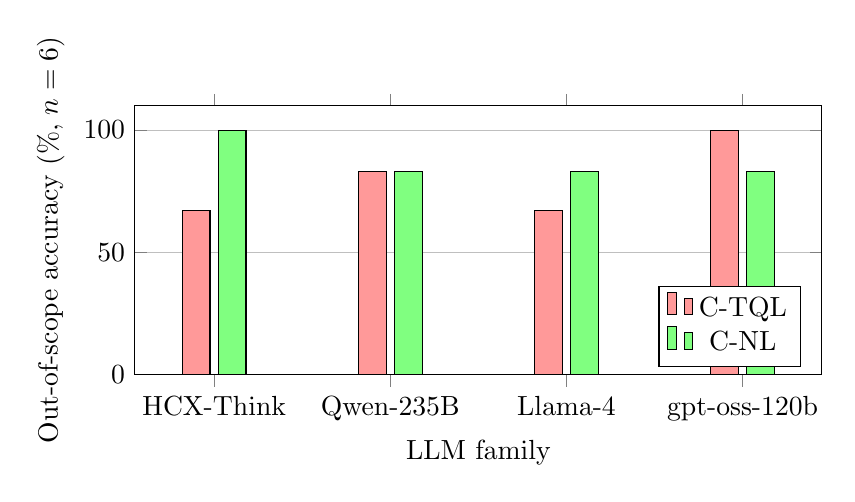
\begin{tikzpicture}
\begin{axis}[
  width=0.85\textwidth,
  height=5cm,
  ybar=3pt,
  bar width=10pt,
  ymin=0, ymax=110,
  ymajorgrids=true,
  ylabel={Out-of-scope accuracy (\%, $n=6$)},
  xlabel={LLM family},
  symbolic x coords={HCX-Think, Qwen-235B, Llama-4, gpt-oss-120b},
  xtick=data,
  legend pos=south east,
  enlarge x limits=0.15,
]
% C-TQL (formal KG)
\addplot[fill=red!40] coordinates {
  (HCX-Think, 67) (Qwen-235B, 83) (Llama-4, 67) (gpt-oss-120b, 100)
};
% C-NL (natural language)
\addplot[fill=green!50] coordinates {
  (HCX-Think, 100) (Qwen-235B, 83) (Llama-4, 83) (gpt-oss-120b, 83)
};
\legend{C-TQL, C-NL}
\end{axis}
\end{tikzpicture}
\caption{Closed-world boundary inference (out-of-scope category, $n=6$).
\textbf{Despite both surface forms containing the same facts}, the
formal KG dump (C-TQL) underperforms natural language (C-NL) on three of
four LLM families. Proving \emph{absence} requires enumeration plus
non-existence verification — a higher cognitive load that compounds with
the lower familiarity of TypeQL syntax. Sample size is small ($n=6$);
this figure is qualitative evidence; per-LLM, per-category breakdowns
are available in the released raw predictions.}
\label{fig:oos}
\end{figure}


Despite full data coverage, the formal KG dumps under-perform
natural language on this category. We attribute this to three
compounding factors:

\begin{enumerate}
\item \textbf{Cognitive load.} A positive lookup requires one
      retrieval. A negative lookup requires \emph{enumerating} all
      candidate facts of the relevant type and verifying that none
      match — a multi-step reasoning chain that is harder under any
      surface form, and especially harder when the syntax is
      unfamiliar.
\item \textbf{Closed-world ambiguity.} A raw KG dump does not signal
      whether absence implies "false" (closed world) or "unknown"
      (open world). The chat model must infer the regime from
      context. Natural-language summary, by contrast, can carry an
      explicit boundary clause — "X is defined only for grades $a$
      and $b$" — verbatim.
\item \textbf{Missing boundary markers.} TypeQL \texttt{insert}
      statements and Cypher \texttt{CREATE} statements are inherently
      assertional: they only express what \emph{is}. There is no
      natural place to assert what \emph{is not}. JSON-LD and
      natural-language summaries have, by contrast, easy linguistic
      affordances for boundary statements.
\end{enumerate}

\subsection{The KG Semantic Paradox}

The two preceding mechanisms compose into what we call the \emph{KG
semantic paradox}. The very strengths that make a KG operationally
valuable — schema-driven structural clarity, explicit role-player
constraints, integrity rules — disappear or invert when the graph is
serialized into an in-context prompt for an LLM. The closed-world
semantics that the operational system relies upon implicitly are
stripped away in raw dumps; the schema constraints are not
reproduced as boundary statements; and the formal query language
that a KG agent could in principle use to express negation
(\texttt{not \{...\};} in TypeQL) is itself the syntactic regime in
which LLMs are weakest. The KG's structural strength becomes its
in-context weakness.

\subsection{Syntax Guides Partially Compensate}

If the bottleneck is query-language familiarity, an
explicit syntax guide should narrow the gap. We test this with
Llama-4-Scout, the model with the largest spread, on C-Cypher (its
weakest formal surface form at 62\%). We prepend a 453-character
syntax primer — three sentences explaining how Cypher's
\texttt{CREATE (var:Label \{prop: value\})-[:REL]->(target)}
notation should be read — and re-run all 100 questions.

\begin{table}[t]
\centering
\caption{Llama-4-Scout on C-Cypher with and without a 453-character
Cypher syntax primer. The guide partially closes the form-sensitivity
gap, with the largest lifts on cross-reference tasks. Out-of-scope
\emph{decreases} (--16.7 pp), suggesting that a syntax guide alone
does not address closed-world boundary inference.}
\label{tab:guide-cypher}
\small
\begin{tabular}{l rrr}
\toprule
Category & C-Cypher & C-Cypher+guide & $\Delta$ \\
\midrule
single\_lookup        & 40.0\% & 60.0\% & $+20.0$ \\
comparison            & 46.2\% & 61.5\% & $+15.4$ \\
aggregation           & 30.0\% & 40.0\% & $+10.0$ \\
calculation           & 92.9\% & 100\%  & $+7.1$  \\
multihop\_3key        & 66.7\% & 73.3\% & $+6.7$  \\
article\_text         & 100\%  & 100\%  & $0$     \\
term\_normalization   & 100\%  & 100\%  & $0$     \\
negation\_exception   & 25.0\% & 25.0\% & $0$     \\
join\_2key            & 60.0\% & 50.0\% & $-10.0$ \\
out\_of\_scope        & 66.7\% & 50.0\% & $-16.7$ \\
\midrule
\textbf{Overall}      & \textbf{62.0\%} & \textbf{67.0\%} & \textbf{$+5.0$} \\
\bottomrule
\end{tabular}
\end{table}

The 5-percentage-point overall lift is non-trivial: it confirms that
syntax familiarity is part of Llama-4's bottleneck, with categories
demanding cross-reference (comparison, single\_lookup,
multihop\_3key) showing the largest individual gains. Tellingly,
\texttt{out\_of\_scope} drops by 16.7 percentage points: a structural
syntax guide is the wrong remedy for closed-world boundary inference.
The two mechanisms are distinct and require distinct interventions.

A 16-percentage-point gap to C-NL (83\%) remains even with the
guide. Syntax familiarity is necessary but not sufficient for closing
the surface-form gap; some additional load — possibly the
cross-reference cognitive cost of formal-syntax reading — persists
beyond what a brief primer can fix.

\paragraph{Guide effectiveness depends on baseline familiarity.}
To probe the limits of the syntax-guide remedy, we repeat the
ablation on C-TQL — the same Llama-4-Scout, the same primer
methodology, a 531-character TypeQL primer explaining N-ary
role-player notation. The result inverts: C-TQL drops from 63\% to
55.8\% (a 7.2-percentage-point regression), with the largest
per-category losses on \texttt{calculation} (--30.2~pp) and
\texttt{join\_2key} (--20.0~pp). Strikingly, the same primer lifts
\texttt{out\_of\_scope} accuracy from 67\% to 100\% (+33.3~pp): the
explicit description of role-player roles seems to prompt the model
to reason about \emph{which} roles are present and absent, but at
the cost of confusing single-fact lookup that was previously working
on syntactic-pattern matching alone.

We read this as evidence that guide remedies are conditional on
baseline syntactic familiarity. Cypher's \texttt{CREATE
(a)-[:R]->(b)} pattern is sufficiently represented in the LLM's
pre-training that a brief primer activates correctly. TypeQL's
N-ary role-player syntax is sufficiently rare that the primer
introduces \emph{new} cognitive load (parsing the guide itself,
re-interpreting prior partial patterns) rather than reinforcing an
existing capability. The implication is that low-familiarity formal
languages may not be repairable from the prompt side at all;
specialized fine-tuning or query-language-aware coder models
(Section~\ref{sec:discussion}, Recommendation~3) are the more
plausible remedy. We treat full coverage of this ablation (four
LLMs $\times$ three structured tiers $\times$ ±guide) as future
work.
